
\subsection{Differenze architetturali: OpenSLES}\label{subsec:mischeWilhelm}
\textit{In questo punto cercherò di difendere l'ipotesi secondo la quale le librerie
interne del sistema operativo Android veicolino indirettamente l'effettuazione
dei controlli sui permessi di sistema.} Quest'occasione viene fornita 
dall'errore riportato dal LogCat durante l'esecuzione di \texttt{pjsua} senza particolari
privilegi utente, ed evidenziato nella Sezione \vref{sec:rootingdevice}. 
In questa sede non descriverò
la libreria OpenSLES, per la quale faccio riferimento alla Sottosezione 
\vref{subsubsec:OnlyAudioOpenSles},
ma metterò in luce il collegamento esistente tra librerie  a supporto
del codice nativo e funzioni di monitoraggio del sistema.

In questa sede mi riferirò ad OpenSLES come ad Wilhelm (\texttt{\small \AOSP/frameworks/wilhelm}),
in quanto in questo punto si effettua l'implementazione di OpenSLES e si forniscono
gli \textit{include} all'interno del percorso \texttt{\small \AOSP/frameworks/wilhelm/include/SLES}.
\medskip




Ripartirò ora con la trattazione facendo riferimento all'analisi degli errori
forniti dal LogCat, e che in particolare fanno riferimento allo strato delle
librerie native. Si può vedere come l'output:
\begin{center}
\textit{ android\_audioRecorder\_realize(...) error creating AudioRecord object}
\end{center}
venga fornito all'interno della funzione \texttt{\small wilhelm} \texttt{\small android\_audioRecorder\_realize}, 
definito nel file \texttt{\small AudioRecorder\_to\_android.cpp}: si può 
immediatamente notare l'invocazione del costruttore \texttt{\small android::AudioRecord()},
il quale in realtà appartiene ad una classe di un'altra libreria, detta \textit{ libmedia},
e definito all'interno del file:
\begin{center}
\texttt{\small \AOSP/frameworks/av/media/libmedia/AudioRecord.cpp}
\end{center}
L'invocazione di tale costruttore implica l'invocazione del metodo \texttt{set},
causando l'invocazione del metodo \texttt{\small openRecord\_l} che è il responsabile
dell'output di errore:
\begin{center}
\textit{ AudioFlinger could not create record track, status: ...}
\end{center}
In particolare questo è il risultato della seguente invocazione:
\begin{cpp}
sp<IAudioRecord> record = audioFlinger->openRecord(getpid(), input, sampleRate, format,channelMask,frameCount,IAudioFlinger::TRACK_DEFAULT,&mSessionId,&status);
\end{cpp}
dove  ci si preoccupa di controllare preventivamente i permessi tramite
l'invocazione del metodo \texttt{\small recordingAllowed()} di \texttt{\small 
ServiceUtilities.cpp}, il quale a sua volta effettua l'invocazione di 
\texttt{\small checkCallingPermission(''android.permission.\\RECORD\_AUDIO'')}.
Il tipo di dato che è definito come \texttt{\small sp} è in particolare l'implementazione
degli \textit{Strong Pointer} che, assieme ai \textit{Weak Pointers} definiti nel file:
\begin{center}
\texttt{\small \AOSP/frameworks/native/libs/utils/RefBase.cpp}
\end{center}
implementano tramite ``smart pointers'' il \textit{Reference Counting}
all'interno del codice C++\footnote{\label{foot:smart}Per non soffermarmi eccessivamente su 
questo aspetto secondario, faccio riferimento
al sito \url{http://www.icepack-linux.com/android-smart-pointer/}}.
È comunque a questo livello, ovvero di libreria \textit{libnbaio}, presente tra altre
all'interno del percorso:
\begin{center}
\texttt{\small \AOSP/frameworks/av/services/audioflinger/}
\end{center}
che noto le prime
chiamate a funzioni della libreria \textit{libbinder}, i cui sorgenti sono situati
all'interno del percorso:
\begin{center}
\texttt{\small \AOSP/frameworks/native/libs/binder/}
\end{center}
Riporto l'inclusione dello header di \texttt{\small ServiceUtilities.cpp}:
\begin{cpp}
#include <binder/IPCThreadState.h>
#include <binder/IServiceManager.h>
#include <binder/PermissionCache.h>
\end{cpp}
\begin{figure}[thp]
\centering
\subfloat[][\textit{Descrizione finale della gerarchia Android. Sono messi in luce i meccanismi di registrazione del servizio e di IPC}.]{\label{subfig:myselfig}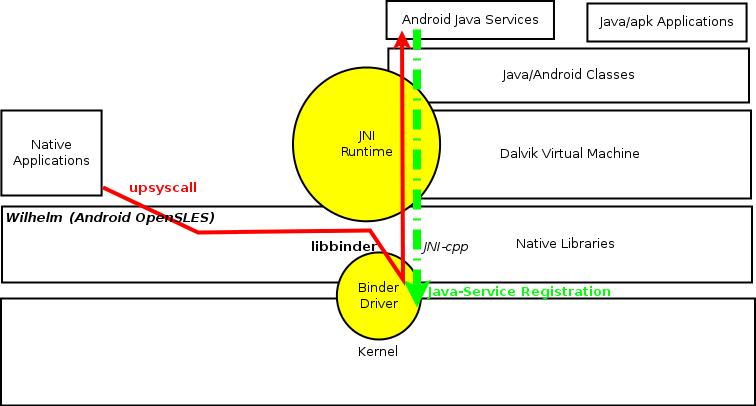
\includegraphics[scale=0.6]{img/modelio/conclus_servandroid.png}}\\
\subfloat[][\hbox{\textit{Visione High-Level dell'architettura Android. \parencite{tesi:binder}}.}]{\label{subfig:genbinder}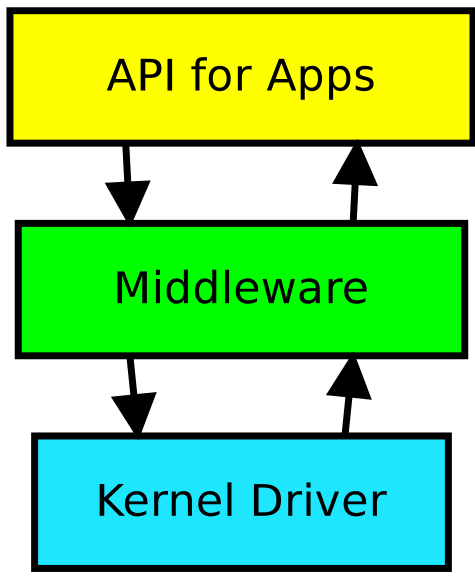
\includegraphics[scale=0.25]{img/teutoinc_level.png}}\\
\caption{Visione dell'interazione tra oggetti interagenti nel corso dell'IPC.}
\label{fig:binderconclusion}
\end{figure}
Sebbene il metodo \texttt{checkCallingPermission} sia definito sia nella classe
\texttt{\small IServiceManager}, sia in \texttt{PermissionCache}, solamente nella prima si
ha l'inclusione di tale metodo all'interno del \textit{namespace} \texttt{android}, che
quindi riporto qui sotto:
\begin{cpp}
bool checkCallingPermission(const String16& permission, int32_t* outPid, int32_t* outUid)
{
    IPCThreadState* ipcState = IPCThreadState::self();
    pid_t pid = ipcState->getCallingPid();
    uid_t uid = ipcState->getCallingUid();
    if (outPid) *outPid = pid;
    if (outUid) *outUid = uid;
    return checkPermission(permission, pid, uid);
}
\end{cpp}

Proseguendo l'analisi dell'output fornito, ottengo che il seguente messaggio:
\begin{center}
\textit{Permission failure: android.permission.RECORD\_AUDIO from uid=10043 pid=2978}
\end{center}
è prodotto ancora una volta dalla classe C++ \texttt{IServiceManager}, della quale
metto in evidenza il codice:
\begin{cpp}
// Is this a permission failure, or did the controller go away?
if (pc->asBinder()->isBinderAlive()) {
   ALOGW("Permission failure: %s from uid=%d pid=%d", String8(permission).string(), uid, pid);
   return false;
}
\end{cpp}
Ciò mostra che effettivamente il Binder è esistente, ma che la restituzione
della chiamata a funzione è \texttt{\small false}.

Ritornando ora a seguire il \textit{fil rouge}, otteniamo che 
la chiamata al \texttt{\small checkPermission} remoto viene garantita dalla chiamata all'omonima
funzione definita all'interno di\\ \texttt{\small IPermissionController}, che effettua
l'inserimento dei dati all'interno del \texttt{Parcel} e richia il metodo:
\begin{cpp}
remote()->transact(CHECK_PERMISSION_TRANSACTION, data, &reply);
\end{cpp}
In questo caso \texttt{\small remote()} non è nient'altro che l'oggetto \texttt{\small mRemote}
\texttt{\small BpBinder} e fornito dal Binder per effettuare la
comunicazione tramite l'omonimo driver, e quindi si riuscirà ad interagire con il
service registrato, che in particolare risponde al descrittore \texttt{\small android.os.IPermissionController}.
Come conclusione posso fornire 
il diagramma degli oggetti proposto in Figura
\vref{fig:binderlowlevel}, palesando così l'effettuazione delle
\textit{upsyscall}.

\begin{java}
static class PermissionController extends IPermissionController.Stub {
        ActivityManagerService mActivityManagerService;
        PermissionController(ActivityManagerService activityManagerService) {
            mActivityManagerService = activityManagerService;
        }

        public boolean checkPermission(String permission, int pid, int uid) {
            return mActivityManagerService.checkPermission(permission, pid,
                    uid) == PackageManager.PERMISSION_GRANTED;
        }
}
\end{java}

Posso quindi ribadire i concetti fin'ora espressi tramite l'ausilio dell'immagine
\subref{subfig:myselfig} \vref{fig:binderconclusion}, che in pratica dettaglia
quello che le fonti avevano già espresso con la Figura \subref{subfig:genbinder}
\vref{fig:binderconclusion}.


